
\chapter{Contexto teórico}

\section{Trading: significado y tipos de análisis}

Como se ha mencionado en el apartado \textit{Motivación} del capítulo \ref{introduccion}, el trading es un concepto que tiene su origen en antiguas civilizaciones de Mesopotamia. \newline


El actual concepto de trading consiste en una práctica aplicada a los mercados financieros. Realizar trading implica comprar o vender dentro de los distintos mercados financieros para vender o comprar de nuevo al cabo de un tiempo y obtener beneficio de la acción realizada. Entre esos activos financieros destacan las acciones de empresas, divisas, materias primas, índices o criptomonedas. \newline

A grandes rasgos y con un ejemplo, realizar trading beneficiosamente podría ser comprar una acción de \textit{Apple} por 100 dólares y venderla en cierto tiempo por 150 dólares, obteniendo por tanto un beneficio de 50 dólares. \newline

\subsection{Tipos de análisis de mercados}

Dada esta introducción a lo que es el trading, vemos obvio que lo que buscamos es maximizar los beneficios cuando ordenamos una compra o una venta. \newline

¿Cuándo se debe comprar o vender un activo? Cuando un operador humano piensa en realizar una operación en el mercado, analiza el activo en cuestión siguiendo una serie de criterios basados en distintos tipos de análisis existentes. \newline

\begin{itemize}
	
	\item \textbf{Análisis fundamental}: El análisis fundamental consiste en operar en base a las distintas noticias que ocurren en el mundo diariamente. Estas noticias sirve de fundamento para actuar de una forma u otra en el mercado. 
	\item \textbf{Análisis técnico}: En este tipo de análisis, el operador o trader opera puramente en base al precio: su acción y movimientos. En este caso, no se tienen en cuenta las noticias. Es este el tipo de análisis interesante a la hora de automatizar. Esto ocurre porque en este método entran en juego cálculos matemáticos como medias, medias móviles, zonas de probabilidad estadística, etc. A partir de este análisis surge el trading algorítmico. \\
	Este análisis, aunque se pueda automatizar, no te asegura que el precio vaya en la dirección resultado del análisis. A pesar de esto, si trabajamos con probabilidades y obtenemos probabilidades de ganar superiores al 50\%, obtendremos un sistema que a largo plazo conseguiría grandes beneficios.
	\item \textbf{Análisis de sentimiento}: En este análisis cobran importancia las opiniones de analistas, prensa u observadores de mercados. Este tipo de análisis ocurre mayormente en el \textit{Forex} (mercado de intercambio de divisas).
	\item \textbf{Análisis macroeconómico}: Análisis en el que se tiene en cuenta el comportamiento y desarrollo de la economía de un país. Tiene relación directa con el \textit{Análisis fundamental} ya que las noticias que más afectan a los mercados suelen ser las de corte económico.
	\item \textbf{Análisis cuantitativo}: Este análisis usa lo que se conoce como matemáticas financieras, concepto que deriva de la física y de la estadística.
\end{itemize} 

\subsection{Principales referentes del análisis de mercados}

A lo largo de la historia moderna, economistas, periodistas y demás personas dedicadas a la inversión han desarrollado una serie de estrategias o métodos de análisis de mercados propios. \newline

En concreto, destacamos los cinco principales referentes del análisis de datos de activos financieros: \textit{Charles Henry Dow}, \textit{Richard Demille Wyckoff}, \textit{William Delbert Gann}, \textit{Ralph Nelson Elliott} y \textit{Arthur Alexander Merrill}. \newline

Estas importantes figuras destacaron por sus avances en el ámbito de la economía y todos fueron importantes analistas de mercados. A continuación, cito a cada uno de dichos economistas en orden descendente de antigüedad con sus principales aportaciones a la materia que nos ocupa. \newline

\textit{Charles Dow} (1851-1902) fue cofundador del periódico \textit{Wall Street Journal}. Entre sus avances en destaca la creación del índice de mercado \textit{Promedio Industrial Dow Jones}. \newline

En el caso de \textit{Richard Wyckoff} (1873-1934), se destaca que fue uno de los pioneros en el análisis técnico de mercados de acciones. \newline

El economista \textit{Elliot} (1871-1948) descubrió que el mercado se basaba en principios sociales subyacentes. A principios de los años 20, concluyó que los mercados siguen las leyes de la naturaleza basándose en ratios de \textit{Fibonacci}. Con esto demostró que el comportamiento de los mercados pueden predecirse.  \newline

\textit{Gann} (1878-1955) destacó por sus métodos de análisis de mercados basados en geometría y matemáticas. Se consideraron técnicas innovadoras y se siguen usando a día de hoy. \newline

Por último, el analista \textit{Arthur Alexander Merrill} (1906-2005) destacó por sus aportes en la creación de un sistema de figuras de precios para ser aplicado en el análisis ténico. \newline

Debido al carácter técnico de los análisis propuestos por cada uno de estos autores, y a su respectiva relevancia, en las siguientes secciones se profundiza sobre los análisis o métodos de \textit{Dow} y \textit{Wyckoff}, como posibles candidatos a ser implementados en la aplicación objetivo de este proyecto. \newline

\subsection{Análisis de Charles Henry Dow}

El método de \textit{Dow} se basa directamente en el precio, que refleja el comportamiento humano. Es el indicador más rápido para confirmar una tendencia y se basa en conceptos sencillos pero efectivos. \newline

Este método consistía en un análisis de máximos y mínimos de las fluctuaciones de los mercados financieros, con objetivo de predecir la dirección del mercado. Estos puntos clave son comparados con los máximos y mínimos anteriores. \newline

Dow desarrollo la siguiente teoría, compuesta de 6 principios y llamada la \textit{Teoría de Dow}: \newline

\begin{enumerate}
	
	\item Cualquier acontecimiento externo (fundamento, noticia, etc.) se ve en el gráfico. En otras palabras, los precios son influenciados por dichas situaciones.
	\item Cada mercado financiero tiene tres etapas o tendencias que se repiten:
	\begin{itemize}
		\item \textbf{Primaria}: tendencia a largo plazo, puede durar entre 1 y 3 años.
		\item \textbf{Secundaria}: tendencia a medio plazo, puede durar entre 3 semanas y 3 meses.
		\item \textbf{Terciaria o menor}: tendencia a corto plazo, dura menos de 3 semanas.
	\end{itemize} 
	\item Cada una de las etapas o tendencias primarias presentan 3 fases, que se pueden presentar de dos formas distintas, según si la tendencia es bajista (el precio tiende a bajar) o alcista (el precio tiende a subir):
	\begin{itemize}
		\item \textbf{Tend. prim. alcista}: acumulación $\rightarrow$ tendencia $\rightarrow$ euforia
		\item \textbf{Tend. prim. bajista}: acumulación $\rightarrow$ tendencia $\rightarrow$ pánico	
	\end{itemize} 
	Estas fases se pueden apreciar en la figura \ref{fases_dow}. \newline
	\begin{figure}[h]
		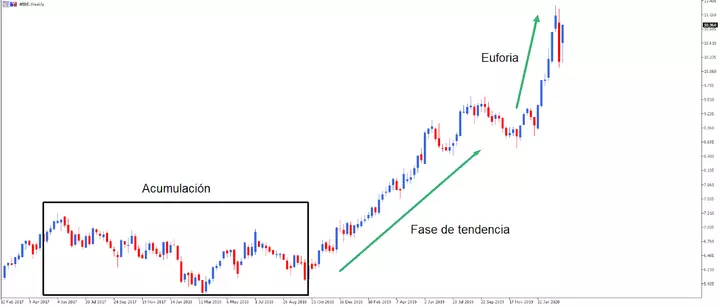
\includegraphics[width=1\textwidth]{imagenes/fases_dow.png} 
		\caption{Fases de acumulación y euforia para tendencia alcista. Fuente: \color{blue} \href{https://admiralmarkets.com/es/education/articles/forex-indicators/teoria-dow}{Teoría de Dow en Análisis Técnico | Dow Theory}} \label{fases_dow}
	\end{figure} \newline
	\item El volumen de negocio confirma la tendencia. El volumen de negocio en trading es la cantidad de un activo en el que se invierte durante un periodo de tiempo. Es un indicador clave de la actividad del mercado y la liquidez.
	\begin{itemize}
		\item Cómo confirma la tendencia alcista: si el precio sube, el volumen aumenta; si el precio baja, el volumen disminuye.
		\item Cómo confirma la tendencia bajista: si el precio sube, el volumen baja; si el precio baja, el volumen aumenta.
	\end{itemize} 
	\item Las tendencias se confirman con los índices \textit{Dow Jones Industrial} y \textit{Dow Jones Transports} (antiguo \textit{Ferrocarril}). Si la tendencia no está confirmada por los índices mencionado tenemos una señal de debilitación de reversión de la tendencia.
	\item La actual tendencia se mantiene vigente hasta que se demuestre el cambio.
	
\end{enumerate} 

En el análisis, Dow considera que en escenarios alcistas se mantiene que tenemos máximos más altos y mínimos más altos. En escenarios bajistas tenemos máximos más bajos y mínimos más bajos. Si no ocurre ni lo primero ni lo segundo, estamos en una situación de mercado lateral o de consolidación. \newline

Dow define en su análisis los siguientes conceptos dentro de los gráficos de precios: \newline

\begin{itemize}
	\item \textbf{Soporte o resistencia:} líneas (o rango) imaginarias en el gráfico de precios que indican zonas. Una vez el precio supera dichas zonas, tenemos una buena posible entrada ya que indica un cambio de tendencia. Indica puntos exactos de entrada al mercado y predice la tendencia.
	\item \textbf{Cascada de mínimos:} la cotización va haciendo mínimos menores. Es una señal de tendencia bajista muy útil para mercados tendenciales con poco retroceso. Se usa un \textit{Stop Lose} más amplio, lo que nos indica un mayor riesgo.
\end{itemize}

Como conclusión, Dow propuso un análisis de mercado para detectar tendencias y períodos de consolidación de los precios. A pesar de que los mercados estén cambiando continuamente, el comportamiento de hoy día en cuanto a dichos conceptos es el mismo que Dow enunció y que recogemos en este apartado.


\subsection{Análisis de Richard Demille Wyckoff}

\textit{Richard Wyckoff} propuso en sus estudios como analista de mercados financieros, un enfoque en 5 pasos:\newline

\begin{enumerate}
	\item Determinar la posición actual y la tendencia futura probable del mercado. Consiste en realizar una evaluación del mercado para ver la tendencia futura y poder tomar decisiones a corto o largo plazo.
	\item Seleccionar acciones en armonía con la tendencia. En tendencia alcista, elegir acciones más fuertes que el mercado, es decir, acciones que produzcan mayores aumentos porcentuales que el mercado durante los repuntes y menores disminuciones durante las reacciones. En el caso de tendencia bajista, acciones más débiles que el mercado.
	\item Elegir operaciones con una causa que iguale o exceda su objetivo mínimo. Aquí entra en juego la ley de Wyckoff de causa y efecto. Se eligen acciones que han creado una causa suficiente para su objetivo. Se utilizan proyecciones Punto y Figura.
	\item Elegir acciones disponibles con respecto a la tendencia o fases de acumulación o distribución.
	\item Elegir un buen activo para operar. Un buen activo será aquel que vaya en armonía con el mercado general, lo que proporcionará más probabilidades de éxito.
\end{enumerate}

Uno de sus principales aportes fueron las tres leyes de su método de análisis, el método Wyckoff:\newline

\begin{enumerate}
	\item \textbf{Ley de oferta y demanda.} Si la demanda es mayor que la oferta, el precio sube; si la demanda es menor que la oferta, el precio baja. El trader o analista debe estudiar el equilibrio de oferta y demanda comparando precio y volumen.
	\item \textbf{Ley de causa y efecto.} La causa se mide con el recuento de volumen en un gráfico. El efecto es la distancia que se mueve el precio correspondiente a dicha causa.
	\item \textbf{Ley de esfuerzo y resultado.} Esta ley proporciona una advertencia de un posible cambio de tendencia en un futuro cercano.
\end{enumerate}


\section{Trading algorítmico}

En pocas palabras, el trading algorítmico es implementar un sistema de trading que opere de forma automática. \newline

El trading algorítmico analiza gráficos de precios de acuerdo a unos criterios preestablecidos, que dependerán del análisis y del propio algoritmo. Cuando el mercado se ajusta a los criterios mencionados, el algoritmo que se ha diseñado para hacer trading ejecutará una acción de compra o venta de manera automática. \newline

Aparte del ahorro de tiempo y esfuerzo, que es la obvia ventaja de usar trading algorítmico, podemos encontrar otros puntos a favor que hacen de las operaciones más eficientes si las comparamos con cómo las haría un operador humano. \newline

\subsection{Ventajas}

\begin{itemize}
	
	\item \textbf{Diversificación}: existe la posibilidad de aplicar un mismo análisis a distintos mercados financieros, aunque puede existir la posibilidad de que en ciertos mercados obtengamos beneficios con una técnica específica que no obtenemos en otro mercado distinto. Esto es más complicado para un operador humano ya que los cambios de acciones de precios en los mercados financieros hacen que un análisis técnico no sea sencillo para un trader acostumbrado a ciertos mercados financieros.
	\item \textbf{Evaluación de técnicas usadas}: debido a que el trading algorítmico automatiza la acción de realizar compras y ventas, podemos evaluar de forma fácil cuándo cierta técnica de análisis es más o menos eficiente en uno u otro mercado. Aquí podemos hablar de distintas horas del día, diferentes temporadas, mercados financieros, etc.
	\item \textbf{Evitar las emociones}: al automatizar un sistema para comprar y vender acciones, el operador humano evita dejarse guiar por las emociones. Esto puede parecer una ventaja simbólica, pero es bastante importante ya que el mercado suele estar sujeto a estadísticas, probabilidades, etc. Si el trader opera suponiendo que cierta vez ocurrirá algo distinto, acaba dejando de lado el análisis puramente técnico. En resumen, evitamos la principal razón por la cual la mayoría de personas que empiezan a dedicarse al trading fracasan, psicología y emociones.
	\item \textbf{Capacidad para desplegar en la nube}: al ser un algoritmo que puede ser desarrollado en un producto software, es posible desplegar o hacer deploy del mismo en un servidor, de manera que el algoritmo desarrollado siempre está conectado al mercado y aplicando reglas para comprar o vender según los criterios mencionados.
	\item \textbf{Precisión y capacidad para realizar compras y ventas de forma simultánea}: el programa sería siempre más preciso que un humano a la hora de realizar entradas y salidas al mercado. Además, puede hacer esto de forma simultánea y operar para distintos mercados financieros a la vez.
	\item \textbf{Posibilidad de aplicar aprendizaje automático}: no sólo podemos centrarnos en desarrollar un algorítmico basado en reglas o análisis del mercado actual sino que también es posible entrenar algoritmos con modelos usando datos históricos de los mercados financieros. Aquí destaca el uso de herramientas de BI y Big Data.
	
\end{itemize}

\subsection{Desventajas}

\begin{itemize}
	
	\item \textbf{Dependencia de noticias}: como se ha mencionado en anteriores apartados de esta memoria, el trading algorítmico surge principalmente del análisis técnico. Aquí destacamos una desventaja del mismo. En el trading algorítmico es muy difícil tener en cuenta noticias que afecten o puedan afectar al comportamiento del mercado en cuestión. Si se decide implementar lógica para estudiar noticias, la complejidad aumenta bastante.
	\item \textbf{Dificultad para detectar la acción del precio}: debido a que el análisis del trading algorítmico es mayoritariamente técnica y basado en cálculos matemáticos, estadística, etc, es complejo detectar la existencia de patrones en el gráfico de precios. Esto sí es más sencillo de realizar por parte de un trader. Entre estos patrones podemos ver soportes, resistencias, líneas de tendencia, niveles, etc. En resumen, es complicado programar una detección de patrones ya que no es algo numérico sino que el operador los identifica a simple vista.
	\item \textbf{Complejidad en la programación}: es realmente complejo programar un algoritmo de trading.
	
\end{itemize}
